\documentclass[xcolor=dvipsnames,9pt]{beamer}
\usepackage{polski}
\usepackage[utf8]{inputenc}
\usepackage{floatflt,graphicx,textcomp, longtable}
\usepackage{hyperref}

% ********** Styl prezentacji **********
\mode<presentation>
{
	\usetheme{PaloAlto}
	\usecolortheme[RGB={18,167,10}]{structure}
}


\author{Anna Jaworska, Radosław Kleczkowski, Piotr Kunowski, Piotr Orłowski}
\institute[Politechnika Gdańska]{opiekun: mgr inż. Tomasz Maria Boiński}

\subject{Projekt grupowy \\ Wizualizacja grafów za pomocą biblioteki Prefuse}
%\AtBeginSubsection[]
%{
	%\begin{frame}<beamer>
		%\frametitle{Plan prezentacji}
		%\tableofcontents
	%\end{frame}
%}

\title[SOVA]{Projekt grupowy \\ Wizualizacja grafów za pomocą biblioteki Prefuse}

\date{04.02.2010}
\logo{\scalebox{0.085}{
\includegraphics{./elementyGraficzne/SOVA.png}}}

\begin{document}

\AtBeginSection[]
{
   \begin{frame}
       \frametitle{}
			\begin{center}
\begin{Huge}
\textcolor{brown}{\textbf{\insertsectionhead}}
\end{Huge}

\end{center}

       %\tableofcontents[currentsection]
   \end{frame}
}

\begin{frame}
	\titlepage
\end{frame}

\begin{frame}
	\frametitle{Agenda}
	\tableofcontents
\end{frame}

\section{Opis projektu}

\begin{frame}
	\frametitle{Opis projektu}
	 \begin{block}{SOVA}
		Simple Ontology Visualization API
	\end{block} 

	\begin{block}{Cel}
		Utworzenie biblioteki w języku Java umożliwiającej wizualizację ontologii zapisanych w OWL API z wykorzystaniem graficznej biblioteki Prefuse. 
	\end{block}
	\begin{block}{Ważne cele funkcjonalne}
		\begin{itemize}
			\item	Intuicyjne API
			\item Dobra dokumentacja
			\item Wizualizacja ontologii
			\item Umożliwienie graficznej edycji i dodawania obiektów OWL API
			\item Udostępnienie informacji do debugowania 
	        \end{itemize}
	\end{block}
\end{frame}


%\begin{frame}
%	\frametitle{Harmonogram - I semestr}
%	\begin{block}{Studium wykonalności}	
%	\begin{itemize}
%		\item  Zlecenie projektowe
% 		\item  Harmonogram
% 		\item Słownik
% 		\item Studium wykonalności
% 	\end{itemize}
% 	\end{block}
% 	\begin{block}{Analiza wymagań}
% 	\begin{itemize}
%  		\item Specyfikacja wymagań
% 	\end{itemize}
% 	\end{block}
% \end{frame}
% 
% \begin{frame}
% 	\frametitle{Harmonogram - I semestr}
% 	\begin{block}{Analiza obiektowa} 
% 	\begin{itemize}
%  		\item Model klas
% 	\end{itemize}
% 	\end{block}
%       \begin{block}{Prototyp} 
% 	\begin{itemize}
%  		\item Prototyp klas
% 	
% 	\end{itemize}
% 	\end{block}
% 	\begin{block}{Odbiór projektu}
% 	\begin{itemize}
%  		\item Plakat
% 		\item Prezentacja
% 	\end{itemize}
% 	\end{block}
% \end{frame}
% 
% 
% \begin{frame}
% 	\frametitle{Harmonogram - II semestr}
% 	\begin{block}{Iteracja 1}
% 	\begin{itemize}
%  		\item Aktualizacja dokumentacji
% 		\item Implementacja
% 		\item Testowanie 
% 	\end{itemize}
% 	\end{block}
% 	\begin{block}{Iteracja 2}
% 	\begin{itemize}
%  		\item Aktualizacja dokumentacji
% 		\item Implementacja
% 		\item Testowanie 
% 	\end{itemize}
% 	\end{block}
% 	\begin{block}{Podsumownie}
% 	\begin{itemize}
%  		\item Aktualizacja dokumentacji
% 		\item Podsumowanie 
% 	\end{itemize}
% 	\end{block}
% \end{frame}

% \section{Studium wykonalności}
% 
% \begin{frame}
% 	\frametitle{Dlaczego?}
% 	\begin{block}{Szukaliśmy odpowiedzi na następujące pytania}
% 		\begin{itemize}
% 		    \item jak należy tworzyć biblioteki w technologii Java
% 		    \item jakich mechnizmów wizualizacji grafów dostarczają biblioteki Java
% 		    \item czy realizacja projektu za pomocą Prefuse jest odpowiednim rozwiązaniem
% 		    \item jaki standard OWL powinien być wspierany przez wytworzony produkt
% 		\end{itemize}
% 	\end{block}
% \end{frame}
% 
% \begin{frame}
% 	\frametitle{Istniejące biblioteki graficzne}
% 	\begin{block}{JUNG (Java Universal Network/Graph Framework)}
% 		\begin{itemize}
% 			\item	wizualizacja danych za pomocą grafów oraz sieci
% 			\item posiada podstawowe algorytmy grafowe
% 			\item BSD
% 	\end{itemize}
% 	\end{block}
% 	\begin{block}{JGraph}
% 		\begin{itemize}
% 			\item	 biblioteka do wizualizacji grafów kompatybilna ze Swingiem
% 				\item posiada podstawowe algorytmy grafowe
% 			\item LGPL
% 	\end{itemize}
% 	\end{block}
% \end{frame}
% 
% \begin{frame}
% 	\frametitle{Istniejące biblioteki graficzne}
% 	\begin{block}{Prefuse}
% 		\begin{itemize}
% 			\item  elastyczna 
% 			\item narzędzia do przechowywania danych
% 			 \item narzędzia do manipulowania danymi 
% 			\item interaktywność wizualizacji 
%                         \item ciągle rozwijana  
% 			\item BSD
% 			\item Wykorzystana w OCS i GrOWL     
% 		\end{itemize}
% 	\end{block}
% 	\begin{block}{Piccolo}
% 		\begin{itemize}
% 			\item	rozbudowany zestaw narzędzi 
% 			\item prespektywa rybiego oka
% 			\item  istnieją trzy wersje: Piccolo.Java, Piccolo.NET oraz PocketPiccolo.NET 
% 			\item wykorzystana w pluginie do Protege o nazwie Jambalaya
% 			\item BSD
% 	\end{itemize}
% 	\end{block}
% \end{frame}


\section{Projekt wizualizacji}

\begin{frame}
	\frametitle{Wizualizacja elementów OWL}
	
\begin{longtable}{lp{7cm}} 

  Thing &
 \scalebox{0.30}{
\includegraphics{./elementyGraficzne/drobne/thing.png}}
 % class.png: 194x86 pixel, 90dpi, 5.48x2.43 cm, bb=0 0 155 69
 \\ 

  Nothing &
 \scalebox{0.30}{
\includegraphics{./elementyGraficzne/drobne/nothing.png}}
 % class.png: 194x86 pixel, 90dpi, 5.48x2.43 cm, bb=0 0 155 69
 \\ 

  Class &
 \scalebox{0.30}{
\includegraphics{./elementyGraficzne/drobne/class.png}}
 % class.png: 194x86 pixel, 90dpi, 5.48x2.43 cm, bb=0 0 155 69
 \\ 

  Individual &
 \scalebox{0.30}{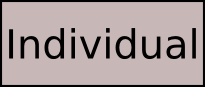
\includegraphics{./elementyGraficzne/drobne/individual.png}}
 % class.png: 194x86 pixel, 90dpi, 5.48x2.43 cm, bb=0 0 155 69
 \\ 

  Property &
 \scalebox{0.30}{
\includegraphics{./elementyGraficzne/drobne/property.png}}
 % class.png: 194x86 pixel, 90dpi, 5.48x2.43 cm, bb=0 0 155 69
 \\ 

  Datatype &
 \scalebox{0.30}{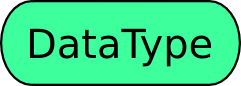
\includegraphics{./elementyGraficzne/drobne/datatype.png}}
 % class.png: 194x86 pixel, 90dpi, 5.48x2.43 cm, bb=0 0 155 69
 \\ 

  Anonymous Class &
 \scalebox{0.30}{
\includegraphics{./elementyGraficzne/drobne/anonymousClass.png}}
 % class.png: 194x86 pixel, 90dpi, 5.48x2.43 cm, bb=0 0 155 69
 \\ 

  Subclass &
 \scalebox{0.30}{
\includegraphics{./elementyGraficzne/drobne/subclass.png}}
 % class.png: 194x86 pixel, 90dpi, 5.48x2.43 cm, bb=0 0 155 69
 \\ 


\end{longtable}
\end{frame}


\begin{frame}
	\frametitle{Wizualizacja elementów OWL}
	
\begin{longtable}{lp{7cm}} 
 instanceOf &
 \scalebox{0.30}{
\includegraphics{./elementyGraficzne/drobne/instanceOf.png}} \newline
 \scalebox{0.30}{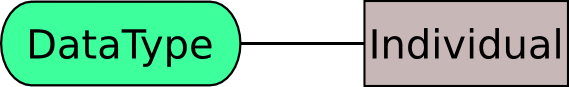
\includegraphics{./elementyGraficzne/drobne/instanceOfDatatype.png}}
 % class.png: 194x86 pixel, 90dpi, 5.48x2.43 cm, bb=0 0 155 69
 \\  

equivalentClass &
 \scalebox{0.30}{
\includegraphics{./elementyGraficzne/drobne/equivalentClass.png}}
 % class.png: 194x86 pixel, 90dpi, 5.48x2.43 cm, bb=0 0 155 69
 \\ 

  disjointWith &
 \scalebox{0.30}{
\includegraphics{./elementyGraficzne/drobne/disjointWith.png}}
 % clas.png: 194x86 pixel, 90dpi, 5.48x2.43 cm, bb=0 0 155 69
 \\ 

  differentFrom / allDifferent &
 \scalebox{0.30}{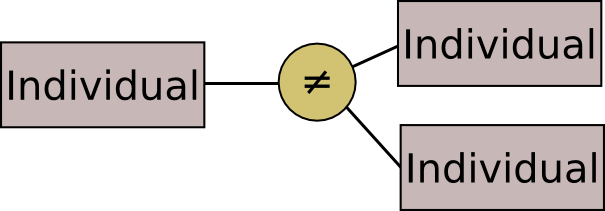
\includegraphics{./elementyGraficzne/drobne/allDifferent.png}}
 % class.png: 194x86 pixel, 90dpi, 5.48x2.43 cm, bb=0 0 155 69
 \\ 

  sameAs &
 \scalebox{0.30}{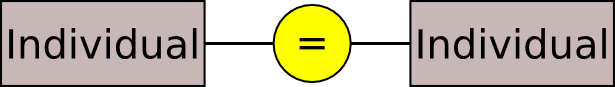
\includegraphics{./elementyGraficzne/drobne/sameAs.png}}
 % class.png: 194x86 pixel, 90dpi, 5.48x2.43 cm, bb=0 0 155 69
 \\ 

\end{longtable}
\end{frame}


\begin{frame}
	\frametitle{Wizualizacja elementów OWL}
	
\begin{longtable}{lp{7cm}} 
 

  oneOf &
 \scalebox{0.30}{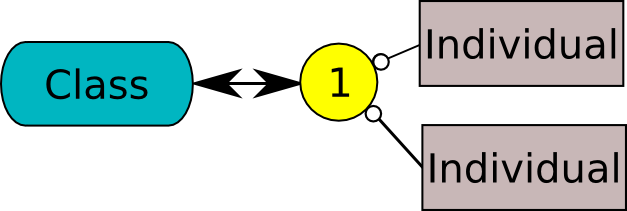
\includegraphics{./elementyGraficzne/drobne/oneOf.png}}
 % class.png: 194x86 pixel, 90dpi, 5.48x2.43 cm, bb=0 0 155 69
 \\ 

  unionOf &
 \scalebox{0.30}{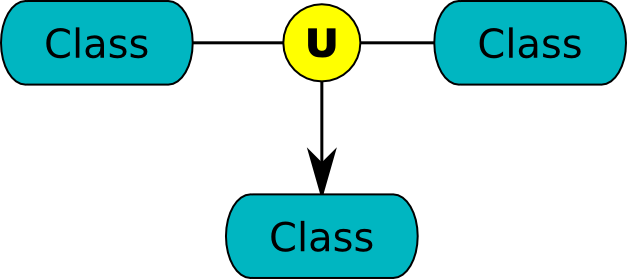
\includegraphics{./elementyGraficzne/drobne/unionOf.png}}
 % class.png: 194x86 pixel, 90dpi, 5.48x2.43 cm, bb=0 0 155 69
 \\ 

  intersectionOf &
 \scalebox{0.30}{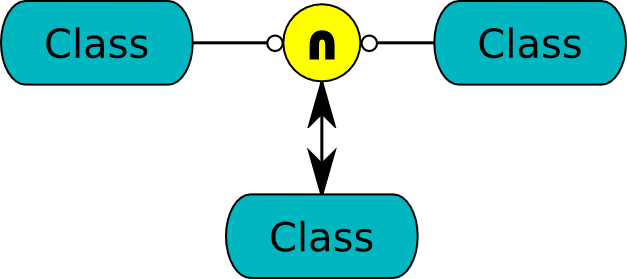
\includegraphics{./elementyGraficzne/drobne/intersectionOf.png}}
 % class.png: 194x86 pixel, 90dpi, 5.48x2.43 cm, bb=0 0 155 69
 \\ 


\end{longtable}
\end{frame}


\begin{frame}
	\frametitle{Wizualizacja elementów OWL}
	
\begin{longtable}{lp{7cm}} 
 

  complementOf &
 \scalebox{0.30}{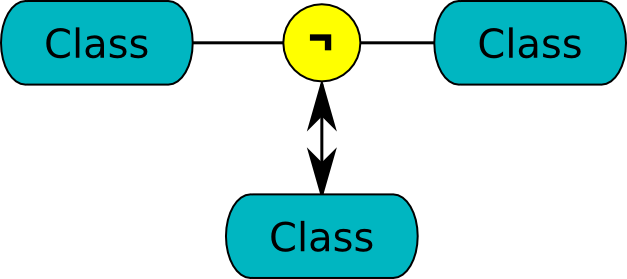
\includegraphics{./elementyGraficzne/drobne/complementOf.png}}
 % class.png: 194x86 pixel, 90dpi, 5.48x2.43 cm, bb=0 0 155 69
 \\ 

  subProperty &
 \scalebox{0.30}{
\includegraphics{./elementyGraficzne/drobne/subProperty.png}}
 % class.png: 194x86 pixel, 90dpi, 5.48x2.43 cm, bb=0 0 155 69
 \\ 

  inverseOf (property) &
 \scalebox{0.30}{
\includegraphics{./elementyGraficzne/drobne/inverseOf.png}} \newline
\scalebox{0.30}{
\includegraphics{./elementyGraficzne/drobne/inverseOfProperty.png}}
 % class.png: 194x86 pixel, 90dpi, 5.48x2.43 cm, bb=0 0 155 69
 \\ 

  equivalentProperty &
 \scalebox{0.30}{
\includegraphics{./elementyGraficzne/drobne/equivalentProperty.png}}
 % class.png: 194x86 pixel, 90dpi, 5.48x2.43 cm, bb=0 0 155 69
 \\ 

\end{longtable}
\end{frame}




\begin{frame}
	\frametitle{Wizualizacja elementów OWL}
	
\begin{longtable}{lp{7cm}} 
 
  functionalProperty &
 \scalebox{0.30}{
\includegraphics{./elementyGraficzne/drobne/functionalProperty.png}}
 % class.png: 194x86 pixel, 90dpi, 5.48x2.43 cm, bb=0 0 155 69
 \\ 

  inverseFunctionalProperty &
 \scalebox{0.30}{
\includegraphics{./elementyGraficzne/drobne/inverseFunctionalProperty.png}}
 % class.png: 194x86 pixel, 90dpi, 5.48x2.43 cm, bb=0 0 155 69
 \\ 

  symmetricProperty &
 \scalebox{0.30}{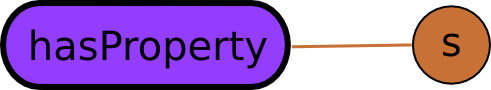
\includegraphics{./elementyGraficzne/drobne/symmetricProperty.png}}
 % class.png: 194x86 pixel, 90dpi, 5.48x2.43 cm, bb=0 0 155 69
 \\ 

  transitiveProperty &
 \scalebox{0.30}{
\includegraphics{./elementyGraficzne/drobne/transitiveProperty.png}}
 % class.png: 194x86 pixel, 90dpi, 5.48x2.43 cm, bb=0 0 155 69
 \\ 

  hasProperty &
 \scalebox{0.25}{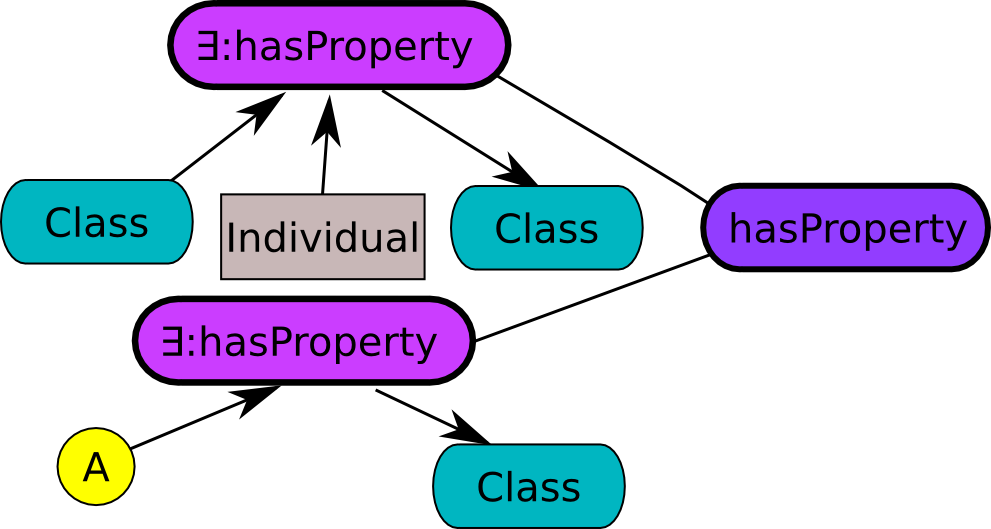
\includegraphics{./elementyGraficzne/drobne/hasProperty3.png}}
 % class.png: 194x86 pixel, 90dpi, 5.48x2.43 cm, bb=0 0 155 69
 \\ 




\end{longtable}
\end{frame}


\begin{frame}
	\frametitle{Wizualizacja elementów OWL}
	
\begin{longtable}{lp{7cm}} 


  allValuesFrom &
 \scalebox{0.25}{
\includegraphics{./elementyGraficzne/drobne/allValuesFrom.png}}
 % class.png: 194x86 pixel, 90dpi, 5.48x2.43 cm, bb=0 0 155 69
 \\ 

  someValuesFrom &
 \scalebox{0.25}{
\includegraphics{./elementyGraficzne/drobne/someValuesFrom.png}}
 % class.png: 194x86 pixel, 90dpi, 5.48x2.43 cm, bb=0 0 155 69
 \\ 
 
 
  domain &
 \scalebox{0.25}{
\includegraphics{./elementyGraficzne/drobne/domain.png}}
 % class.png: 194x86 pixel, 90dpi, 5.48x2.43 cm, bb=0 0 155 69
 \\ 

  range &
 \scalebox{0.25}{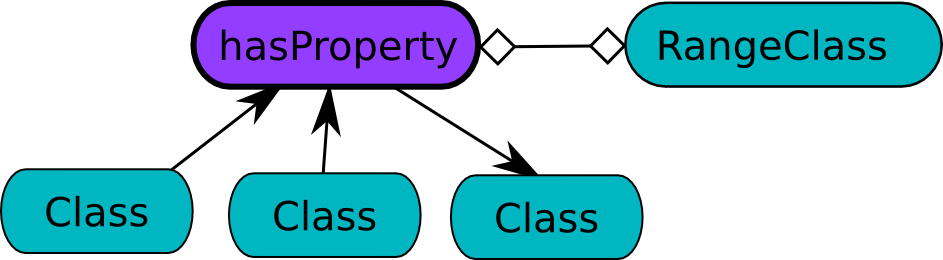
\includegraphics{./elementyGraficzne/drobne/range.png}}
 % class.png: 194x86 pixel, 90dpi, 5.48x2.43 cm, bb=0 0 155 69
 \\ 


\end{longtable}
\end{frame}

\begin{frame}
	\frametitle{Wizualizacja elementów OWL}
	
\begin{longtable}{lp{7cm}} 


  minCardinality / maxCardinality &
 \scalebox{0.30}{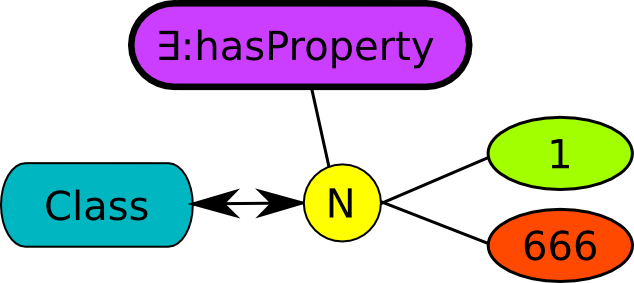
\includegraphics{./elementyGraficzne/drobne/cardinalityminmax.png}}
 % class.png: 194x86 pixel, 90dpi, 5.48x2.43 cm, bb=0 0 155 69
 \\ 

  cardinality &
 \scalebox{0.30}{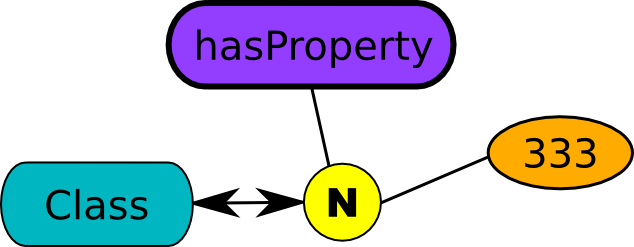
\includegraphics{./elementyGraficzne/drobne/cardinality.png}}
 % class.png: 194x86 pixel, 90dpi, 5.48x2.43 cm, bb=0 0 155 69
 \\ 


\end{longtable}
\end{frame}


\section{Prezentacja produktu} 
% 
% \begin{frame}[plain]
% 	 \scalebox{0.55}{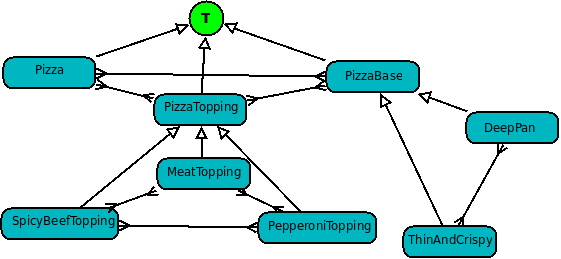
\includegraphics{./elementyGraficzne/tutorialProtege/4-3Class.png}}
% \end{frame}
% 
% \begin{frame}[plain]
% 	 \scalebox{0.60}{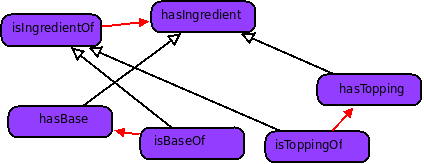
\includegraphics{./elementyGraficzne/tutorialProtege/4-5property.png}}
% \end{frame}
% 
% \begin{frame}[plain]
% 	 \scalebox{0.350}{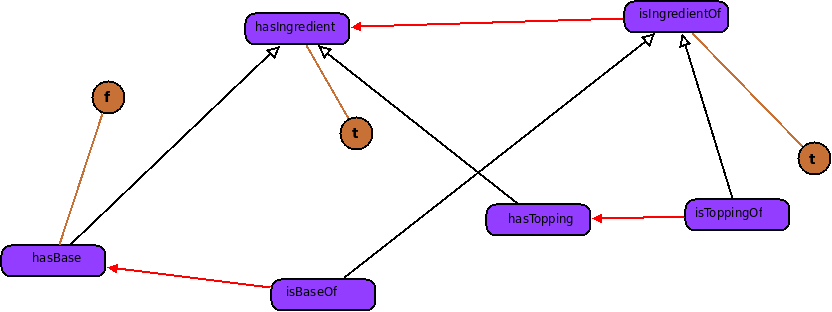
\includegraphics{./elementyGraficzne/tutorialProtege/4-6property2.png}}
% \end{frame}
% 
% \begin{frame}[plain]
% 	 \scalebox{0.2}{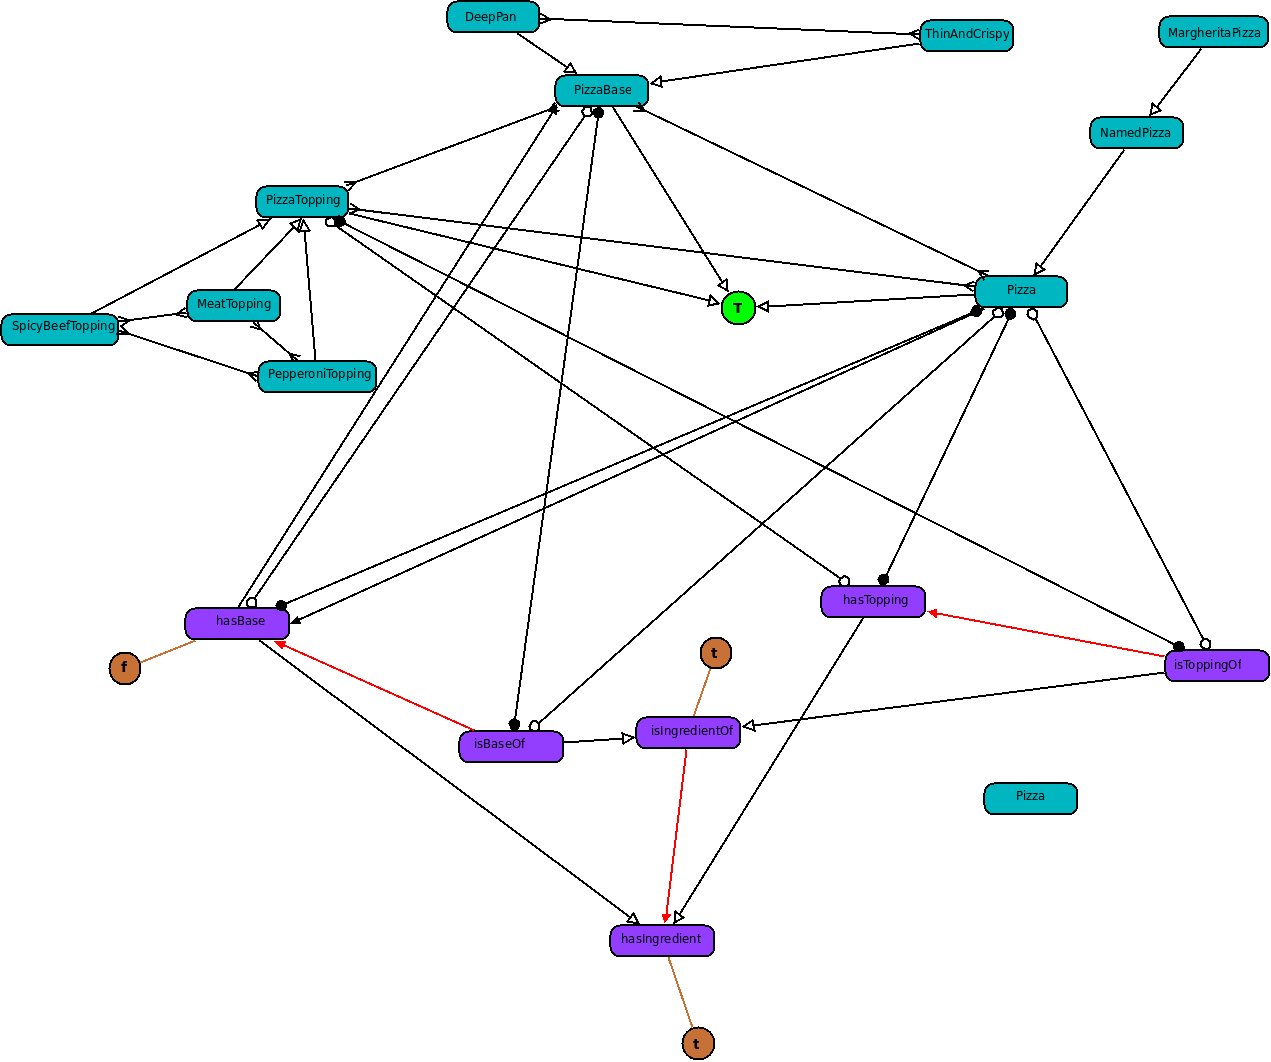
\includegraphics{./elementyGraficzne/tutorialProtege/4-7property2.png}}
% \end{frame}
% 
% \begin{frame}[plain]
% 	 \scalebox{0.20}{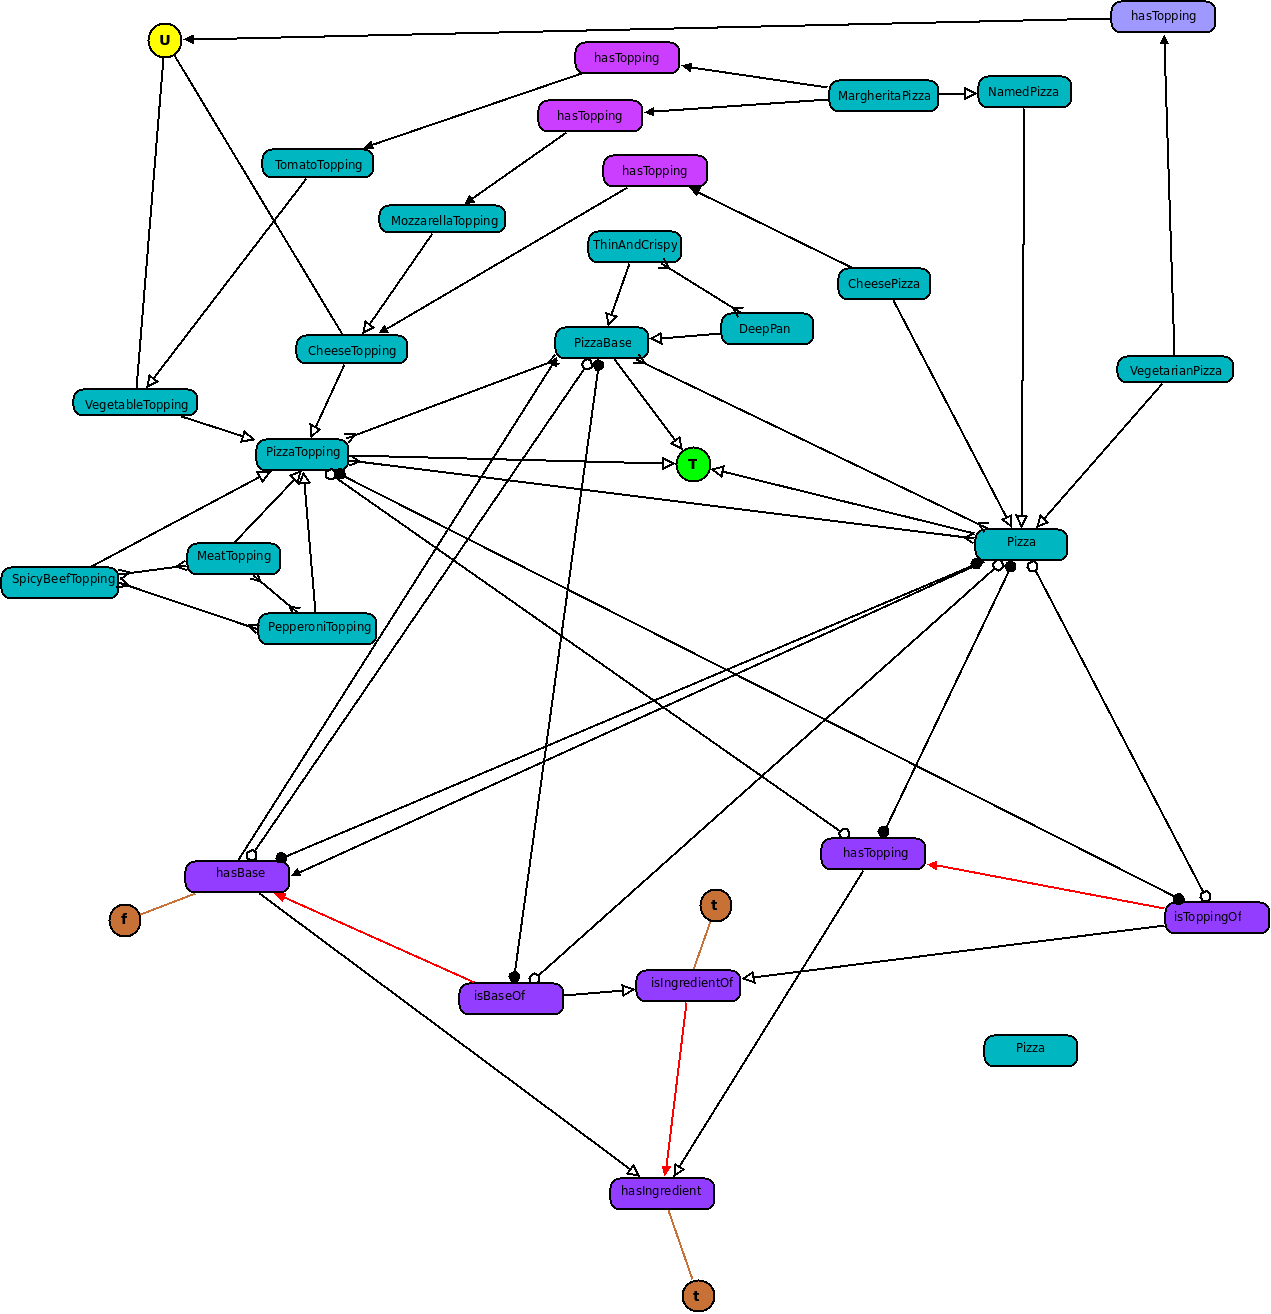
\includegraphics{./elementyGraficzne/tutorialProtege/wszystko(cw31).png}}
% \end{frame}
% 

\section{Podsumowanie projektu}

\begin{frame}
	\frametitle{Osiągnięte cele}

\begin{block}{Cele zrealizowane}
		\begin{itemize}
			\item Intuicyjne API
			  \item Dobra dokumentacja
			\item Wizualizacja ontologii 
			\item Udostępnienie informacji do debuggowania 
	\end{itemize}
	\end{block}




	\begin{block}{Cele poza zakresem projektu}
		\begin{itemize}
			\item Umożliwienie graficznej edycji i dodawania obiektów OWL API
	\end{itemize}
	\end{block}


\end{frame}


\begin{frame}
	\frametitle{Zrealizowane wymagania}
	

	\begin{block}{Wymagania wizualizacji}
	\begin{itemize}
			
			\item Rozróżnialność podstawowych symboli
			\item Rozróżnialność szczególnych typów Class
			\item Rozróżnialność związków między klasami (Class), instancjami (Individual) oraz predykatami (Property)
			\item Rozróżnialność ograniczeń predykatów (Restrictions)
			\item \textbf{Wizualizacja została zaimplementowany zgodnie z projektem} 
	\end{itemize}
	\end{block}

	\begin{block}{Inne istotne zrealizowane wymagania}
	\begin{itemize}
			\item Parametryzacja trybów wizualizacyjnych
			\item Obsługa obiektów OWL API
			\item Poprawność wizualizacji
			\item Kompletność wizualizacji
			\item Dokumentacja w javadoc
			\item Dokumentacja w języku polskim
	\end{itemize}
	\end{block}
\end{frame}

\begin{frame}
	\frametitle{Niezrealizowane wymagania}

	\begin{block}{Wymagania wizualizacji}
		\begin{itemize}
			\item Podświetlanie wybranych związków i powiazań
			 \item Możliwość definiowania zdarzeń - wymaganie poza zakresem projektu
	\end{itemize}
	\end{block}
  	
	\begin{block}{Inne wymagania}
	\begin{itemize}
			\item Dokumentacja w języku angielskim
	\end{itemize}
	\end{block}



\end{frame}

\section{Sukces?}





\end{document}

